\documentclass[12pt]{article}
\usepackage{setspace}
\usepackage{mathpazo}
\usepackage{graphicx}
\usepackage{color}
\definecolor{darkblue}{rgb}{.05,.05,.30}
\usepackage{url}
\usepackage{hyperref}
\hypersetup{pdfborder=0 0 0, colorlinks=true, citecolor=black, linkcolor=black, urlcolor=darkblue, letterpaper}
\usepackage{tikz}
\usetikzlibrary{matrix,arrows,positioning}
%\usepackage{arabtex}
%\usepackage{utf8}
%% For ArabTeX
%\setcode{utf8}
%\setfarsi

\pagestyle{empty}

\begin{document}
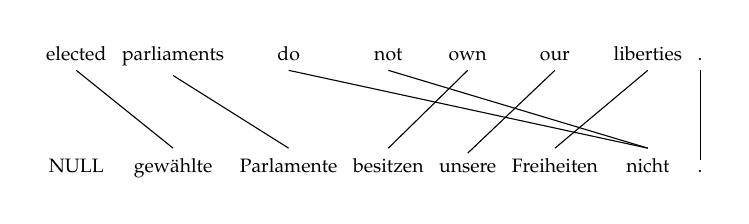
\begin{tikzpicture}
  \pgfsetmatrixcolumnsep{-0.1em}
    %\matrix (eg) [matrix of nodes,anchor=,ampersand replacement=\&,font=\scriptsize]
    \matrix (eg) [matrix of nodes,font=\scriptsize]
  {
	elected & parliaments & do & not & own & our & liberties & . \\
    \mbox{} \\[2em]
	NULL & gew\"{a}hlte & Parlamente & besitzen & unsere & Freiheiten & nicht & . \\
	%NULL ({ }) gewählte ({ 1 }) Parlamente ({ 2 }) besitzen ({ 5 }) unsere ({ 6 }) Freiheiten ({ 7 }) nicht ({ 3 4 }) . ({ 8 })
  };
	\draw[-] (eg-1-1.south) to (eg-3-2.north);
	\draw[-] (eg-1-2.south) to (eg-3-3.north);
	\draw[-] (eg-1-5.south) to (eg-3-4.north);
	\draw[-] (eg-1-6.south) to (eg-3-5.north);
	\draw[-] (eg-1-7.south) to (eg-3-6.north);
	\draw[-] (eg-1-3.south) to (eg-3-7.north);
	\draw[-] (eg-1-4.south) to (eg-3-7.north);
	\draw[-] (eg-1-8.south) to (eg-3-8.north);
\end{tikzpicture}
\end{document}
